\documentclass[letterpaper]{article}

\setlength{\textheight}{8.875in}
\setlength{\topmargin}{0in}
\setlength{\headheight}{0in}

\usepackage{booktabs}
\usepackage{makecell}
\usepackage{float,graphicx}
\usepackage[breaklinks=true,hidelinks]{hyperref}
\appto\UrlBreaks{\do\-}

\begin{document}
	\title{Homework Assignment 1}
	
	\author{Ethan Chung\\
		{\tt\small University of Hawaii}\\
		{\tt\small ICS 635: Machine Learning}\\
		{\tt\small [redacted]@hawaii.edu}}

	{\def\null\vskip 2em{}\maketitle}
	
	\section{Task Description}
	
		The objective of this assignment is to implement and evaluate the performance of three machine learning models (K-Nearest Neighbors (KNN), Decision Trees (DT), and Random Forest (RF)) using the Breast Cancer dataset available within the scikit-learn  library.
	
	\section{Model Description}
	
		K-Nearest Neighbors (KNN) is a supervised learning algorithm that classifies data points based on the majority class among their \textbf{k} nearest neighbors. KNN stores the training data and calculates distances during prediction. Decision Trees (DT) are tree-based models that recursively partition data based on feature values, and are easy to interpret but prone to overfitting. Random Forests (RF) are ensemble methods that combine multiple decision trees, which improve robustness and reduce overfitting through bagging and feature randomness.
	
	\section{Experiment Settings}
	
	\subsection{Dataset Description}
	
		The Breast Cancer dataset, sourced from scikit-learn, is used in this assignment.  It is a binary classification dataset containing 569 samples, each belonging to one of two classes: malignant (212 samples) or benign (357 samples). The dataset comprises 30 features that describe the cells, like radius, texture, perimeter, etc. The dataset was partitioned into training and testing sets using scikit-learn's \texttt{train\_test\_split} function with an 80/20 split for training and test set.
	
	\subsection{Experimental Setup}
	
		Three classifiers were created: KNN, DT, RF, initially with default parameters from scikit-learn. For KNN only, the features are first standardized by removing the mean and scaling to unit variance. Afterwards, all three models were fit on the training set, then evaluated on the test set. Hyper-parameters were tested following this configuration, with the 0th index as the default parameters:
		
		\begin{verbatim}
			knn_n_neighbors = [5, 10, 15, 20, 30]
			dt_max_depth = [None, 1, 5, 10, 20]
			rf_n_estimators = [100, 200, 300, 400, 500]
			rf_max_depth = [None, 1, 5, 10, 20]
			rf_min_samples_split = [2, 4, 6, 8, 10]
		\end{verbatim}
	
	\subsection{Evaluation Metrics}
	
		Accuracy, Precision, Recall, F1 score is used as the evaluation metrics. Accuracy is the proportion of correctly classified instances out of the total instances  Precision is the proportion of correctly classified positive instances out of the total instances classified as positive, which helps measure the accuracy of positive predictions. Recall is the proportion of actual positive instances out of the total instances correctly classified as positive and falsely classified as negative. F1 score is the harmonic mean between precision and recall. A confusion matrix is generated to visualize the TP/FP/TN/FN rates. Using these four metrics together is good for binary classifications that also contain an imbalanced dataset.
		
	\subsection{Source Code}
		\url{https://github.com/echung32/ics635/tree/main/hw1}
	
	\subsection{Model Performance}
	
		Table \ref{tab:model_performance} summarizes the performance of the three models, including the results obtained after tuning various hyperparameters (see Section \ref{ablation} for details). The performance achieved using scikit-learn's default hyperparameters is indicated in \textit{italics}, where Random Forest demonstrated the best performance with an accuracy of 93.85\%, while KNN achieved 96.49\% and Decision Tree 87.71\%.

	\subsection{Ablation Studies} \label{ablation}
	
		Table \ref{tab:model_performance} includes the hyper-parameter tuning experiment results. 
	
		\begin{itemize}
			\item \textbf{KNN:} Larger values of \texttt{n\_neighbors} had a negative impact on accuracy, likely due to the inclusion of less relevant neighbors in the classification. Thus, the highest accuracy achieved was on the default model.
			
			\item \textbf{Decision Tree:} Adjusting \texttt{max\_depth} had limited effect, until \texttt{max\_depth=20} which improved accuracy by 3.51\% compared to the default model. 
			
			\item \textbf{Random Forest:} The best performance was achieved with \texttt{n\_estimators=400, max\_depth=10, min\_samples\_split=8}. However, because these three hyperparameters were varied simultaneously, it is difficult to isolate the individual impact of each on the observed performance improvement.
		\end{itemize}
		
	\section{Conclusion}
	
		This report evaluated KNN, Decision Tree, and Random Forest models on the Breast Cancer dataset using accuracy, precision, recall, and F1-score. Initial runs with default hyperparameters showed Random Forest performing best (93.85\% accuracy), followed by KNN (96.49\%) and then Decision Tree (87.71\%). Hyperparameter tuning revealed that larger \texttt{n\_neighbors} for KNN decreased accuracy, while increasing \texttt{max\_depth} for Decision Tree improved performance, with the best model achieving 91.22\% accuracy. Random Forest also benefited from tuning \texttt{n\_estimators, max\_depth, min\_samples\_split}, with the best model achieving 95.61\% accuracy. 
		
		While hyperparameter tuning improved the performance of both the Decision Tree and Random Forest models, the default KNN model achieved the best accuracy of 96.49\% on this dataset. This suggests that, for this specific dataset, the simpler KNN model generalized well to unseen data.
		
	\section{Figures \& Tables}
	
	\begin{table}[htbp]
		\centering

			\begin{tabular}{lcccc}
				\toprule
				Model & Accuracy & Precision & Recall & F1-Score \\
				\midrule
				\midrule
				KNN & & & & \\
				\midrule
				\textbf{\textit{n\_neighbors=5}} & 0.964912 & 0.968750 & 0.962963 & 0.964640 \\
				n\_neighbors=10 & 0.956140 & 0.961538 & 0.953704 & 0.955728 \\
				n\_neighbors=15 & 0.938596 & 0.947761 & 0.935185 & 0.937787 \\
				n\_neighbors=20 & 0.929825 & 0.941176 & 0.925926 & 0.928750 \\
				n\_neighbors=30 & 0.929825 & 0.941176 & 0.925926 & 0.928750 \\
				\midrule
				Decision Tree & & & &  \\
				\midrule
				\textit{max\_depth=None} & 0.877193 & 0.877792 & 0.875926 & 0.876585 \\
				max\_depth=1 & 0.850877 & 0.857256 & 0.847222 & 0.848912 \\
				max\_depth=5 & 0.877193 & 0.877792 & 0.875926 & 0.876585 \\
				max\_depth=10 & 0.877193 & 0.877792 & 0.875926 & 0.876585 \\
				\textbf{max\_depth=20} & 0.912281 & 0.912037 & 0.912037 & 0.912037 \\
				\midrule
				Random Forest & & & &  \\
				\midrule
				\textit{\makecell[l]{n\_estimators=100, \\ max\_depth=None, \\ min\_samples\_split=2}} & 0.938596 & 0.938213 & 0.938889 & 0.938478 \\
				\makecell[l]{n\_estimators=200, \\ max\_depth=1, \\ min\_samples\_split=4} & 0.929825 & 0.930831 & 0.928704 & 0.929477 \\
				\makecell[l]{n\_estimators=300, \\ max\_depth=5, \\ min\_samples\_split=6} & 0.938596 & 0.938911 & 0.937963 & 0.938364 \\
				\textbf{\makecell[l]{n\_estimators=400, \\ max\_depth=10, \\ min\_samples\_split=8}} & 0.956140 & 0.956542 & 0.955556 & 0.955974 \\
				\makecell[l]{n\_estimators=500, \\ max\_depth=20, \\ min\_samples\_split=10} & 0.938596 & 0.938911 & 0.937963 & 0.938364 \\
				\bottomrule
			\end{tabular}%

		\caption{Classification performance of various models at varying hyper-parameters, as evaluated on the held-out test set. \textit{Italicized} is the default parameters. \textbf{Bolded} are the best performing models.}
		\label{tab:model_performance}
	\end{table}
	
	\begin{figure}[H]
		\centering
		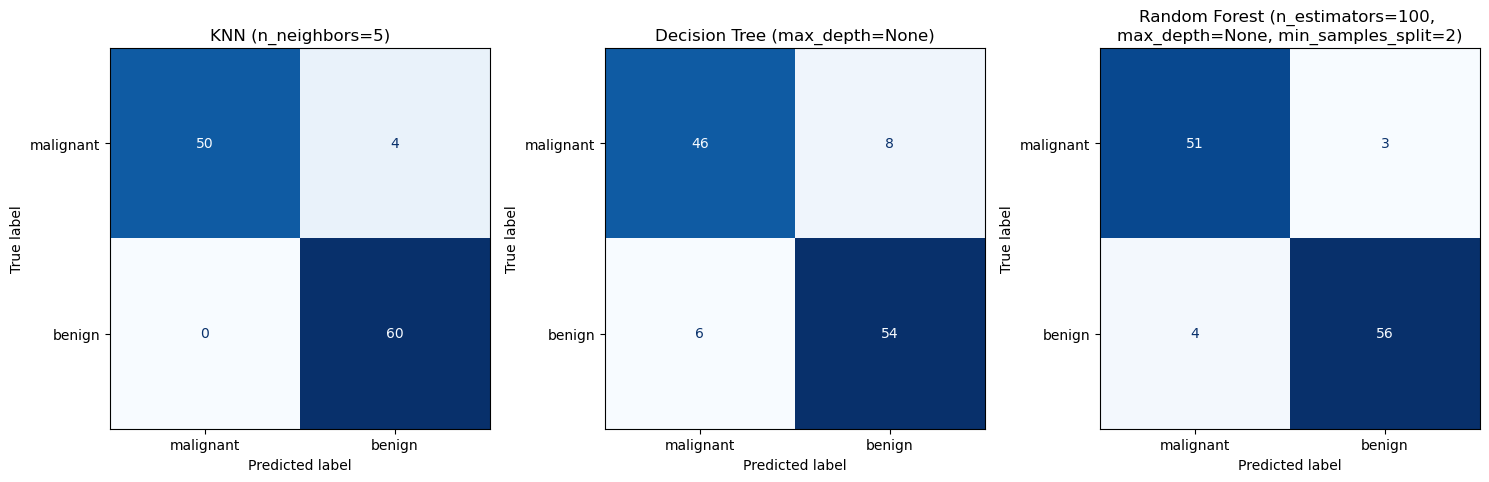
\includegraphics[width=1\linewidth]{figures/1}
		\caption{Default Model Performance}
		\label{fig:1}
	\end{figure}
	
	\begin{figure}[H]
		\centering
		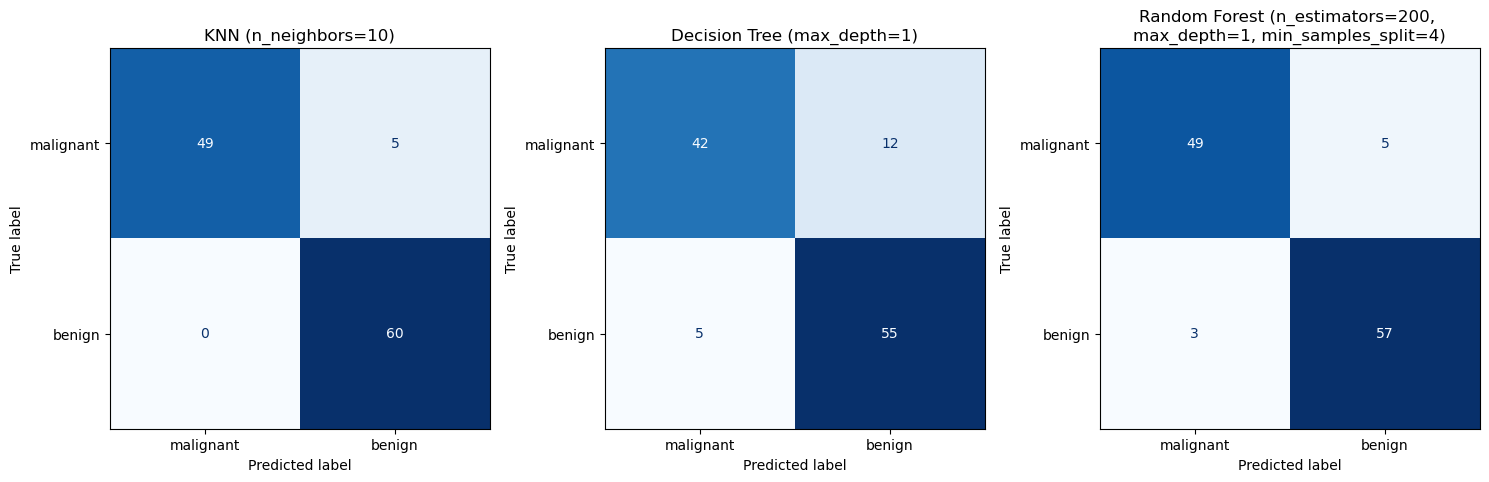
\includegraphics[width=1\linewidth]{figures/2}
		\caption{Ablation Model 1}
		\label{fig:2}
	\end{figure}
	
	\begin{figure}[H]
		\centering
		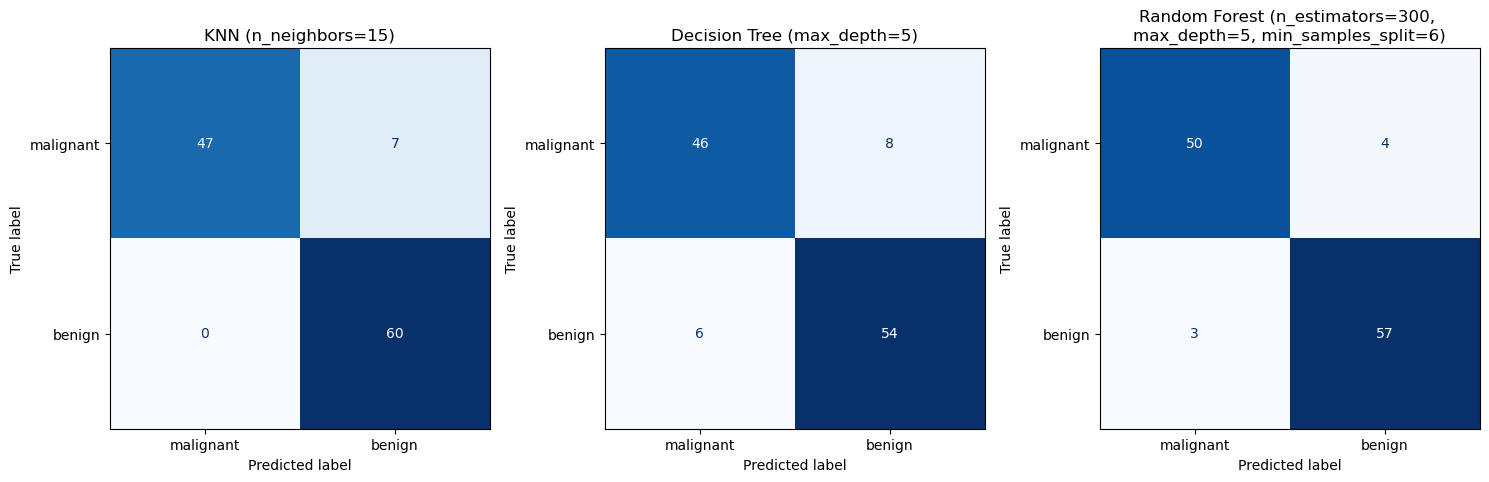
\includegraphics[width=1\linewidth]{figures/3}
		\caption{Ablation Model 2}
		\label{fig:3}
	\end{figure}
		
	\begin{figure}[H]
		\centering
		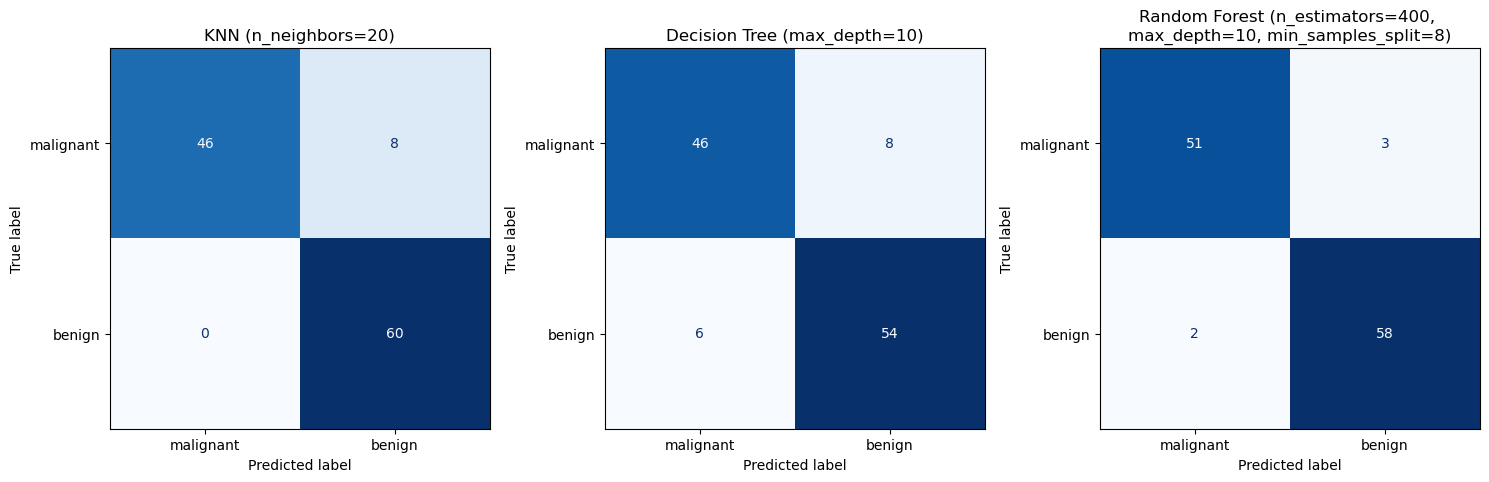
\includegraphics[width=1\linewidth]{figures/4}
		\caption{Ablation Model 3}
		\label{fig:4}
	\end{figure}
		
	\begin{figure}[H]
		\centering
		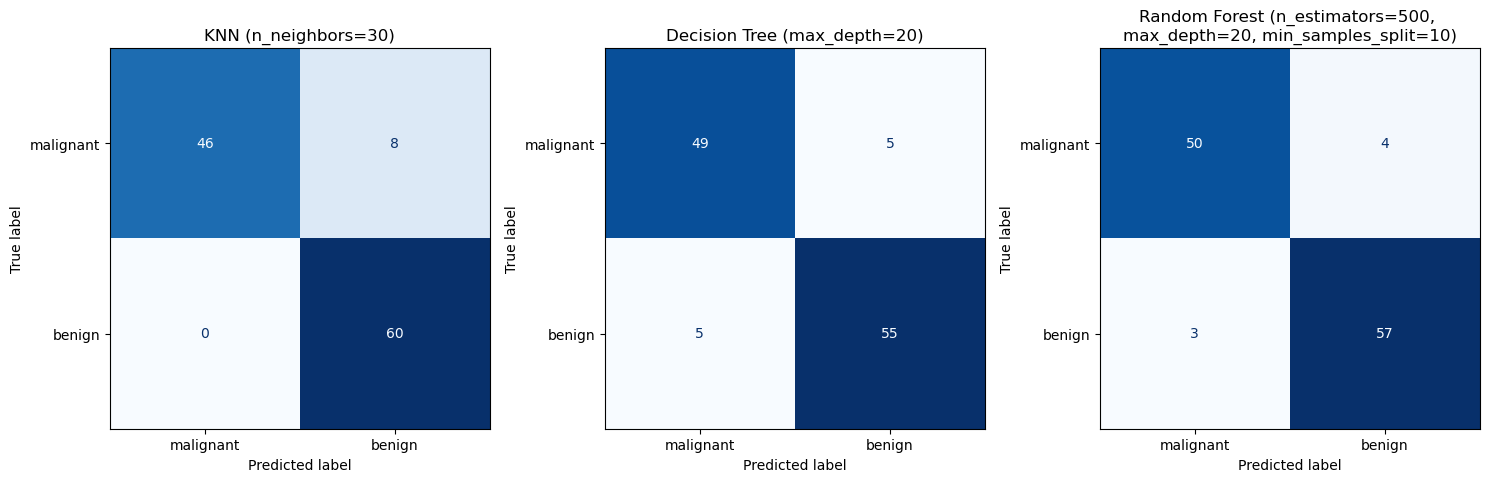
\includegraphics[width=1\linewidth]{figures/5}
		\caption{Ablation Model 4}
		\label{fig:5}
	\end{figure}
	
\end{document}